\documentclass{standalone}

\usepackage{graphicx}
\usepackage{tikz}
\usepackage{tikzsymbols}
\usetikzlibrary{calc}
\usepackage{float}
\usepackage{pdflscape}

\def\centerarc[#1](#2)(#3:#4:#5){\draw[#1] ($(#2)+({#5*cos(#3)},{#5*sin(#3)})$) arc (#3:#4:#5);}

\pagestyle{empty}
\begin{document}
%    \centering
%	\begin{figure}[H]
		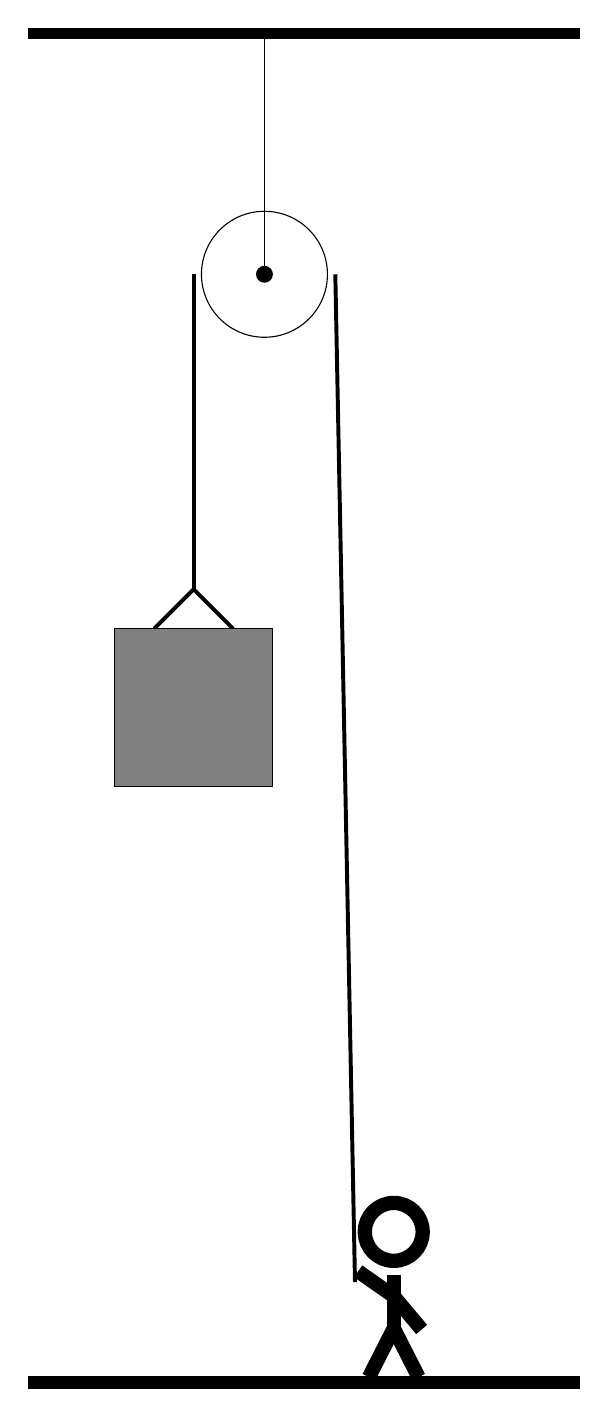
\begin{tikzpicture}
			%%%%% START %%%%%
			\def\a{14}
			\def\radlg{0.8}
			\def\radrp{0.9}
			\def\radsm{0.1}
			\def\yone{\a-3}
			\def\xone{1}
			\def\dxtwo{9}
			\def\dx{2.6}
			\def\dy{-1.9}
			\def\dw{1.75mm}
			\def\hlena{\a*0.5}
			\def\width{0.5mm}
			
			\draw[fill=black] (-2,\a) rectangle (5,\a+0.125);
			
			\draw (\xone,\yone) circle (\radlg);
			\draw[fill=black] (\xone,\yone) circle (\radsm);
			\draw (\xone,\a) -- (\xone,\yone);
			
			\draw[line width=\width] (\xone-0.5-\radrp,\a-\hlena-0.5) -- (\xone-\radrp,\a-\hlena) -- (\xone+0.5-\radrp,\a-\hlena-0.5);
			\draw[fill=black!50] (\xone-1-\radrp,\a-\hlena-0.5) rectangle (\xone+1-\radrp,\a-\hlena-2-0.5); 

			\draw[line width=\width] (\xone-\radrp,\yone) -- (\xone-\radrp,\a-\hlena);
			\centerarc[line width=\width](\xone,\yone)(0:180:\radrp);
			\draw[line width=\width](\xone+\radrp,\yone) -- (\dx-0.45,\dy+0.1);

			\node at (\dx,\dy) {\Strichmaxerl[10][-35][-50]};
			
			\draw[fill=black] (-2,-3) rectangle (5,-3.15);
			%%%%% END %%%%%
		\end{tikzpicture}
%	\end{figure}
\end{document}

